% Provenance (never printed): cycle 4 SVT, "La planete Terre, l'environnement
% et l'action humaine": the relief as a balance between uplift and erosion;
% landforms of the wind, the sea and dissolution; reading a landscape; see
% sources/book1/PROVENANCE.md. Book 1, grade 9, chapter 4.
% Vocabulary guard: owns uplift, dune, cliff, beach and spit (with longshore
% drift), karst (with cave and sinkhole). Landscape and landform are g1's;
% weathering, erosion, deposition, meander and delta are g5's; relief is
% g4's; plates and mountain building are g7's; U-shaped valley and moraine
% are g8's; limestone and the acid test are g6's; acids are the chemistry
% books' (recalled in prose). Contour lines are g9.5's (not used here).
% "Normal fault" and the destruction of mountains are Book 2's.
\chapter{स्थलरूप}\label{ch:g9:landforms}

इंग्लैंड के दक्षिणी \omterm{def:g1:landscapes-around-us:water}{तट} पर सेवन सिस्टर्स की सफ़ेद \omterm{def:g9:landforms:cliff}{कगारें} सीधे \omterm{def:g2:water-on-earth:ocean}{समुद्र} में गिरती हैं। एक सामान्य
वर्ष में वे एक मीटर तक खो देती हैं। 2014 के जाड़े में \omterm{def:g5:natural-hazards:storm}{तूफ़ानों} ने बर्लिंग गैप पर \omterm{def:g9:landforms:cliff}{कगारों} से दो
महीनों में उतना ले लिया जितना वे आमतौर पर सात वर्षों में खोती हैं। इन \omterm{def:g9:landforms:cliff}{कगारों} का खड़िया कभी
किसी \omterm{def:g2:water-on-earth:ocean}{समुद्र} के तल पर \omterm{def:g3:stones-pebbles-sand:sand}{कीचड़} था, जो उसके पानी में रहने वाले सूक्ष्म शैवालों की नन्ही पट्टिकाओं
से बना था। आज वह सफ़ेद \omterm{def:g3:stones-pebbles-sand:rock}{चट्टान} की एक दीवार की तरह खड़ा है जिसे लहरें हर वर्ष थोड़ा और पीछे
काटती हैं। ज़मीन के वे आकार क्यों हैं जो हैं, और उनमें से कुछ इतनी तेज़ी से क्यों बदलते
हैं?
% ledger: nt:birling-2014, sdnp:birling, nasa:coccoliths

\begin{omfigure}
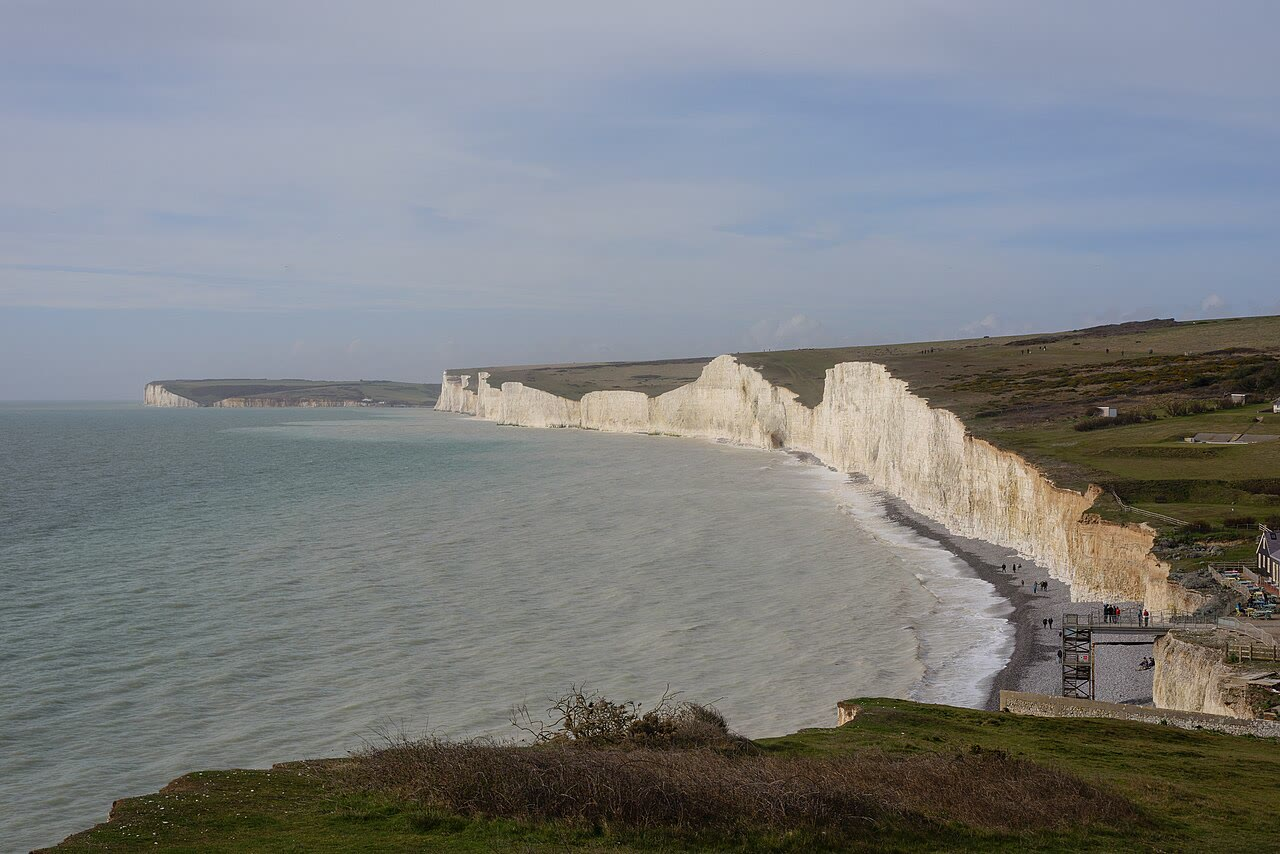
\includegraphics[width=\linewidth]{images/book1/g9-seven-sisters.jpg}

{\small सेवन सिस्टर्स, ईस्ट ससेक्स (इंग्लैंड) के \omterm{def:g1:landscapes-around-us:water}{तट} पर खड़िया की \omterm{def:g9:landforms:cliff}{कगारें}, अग्रभूमि में
बर्लिंग गैप के घरों के साथ। \omterm{def:g9:landforms:cliff}{कगारों} को \omterm{def:g2:water-on-earth:ocean}{समुद्र} पीछे काटता है, और \omterm{def:g3:stones-pebbles-sand:rock}{चट्टानें} किसी भी समय गिर
सकती हैं। उनके तल पर \omterm{def:g3:stones-pebbles-sand:pebble}{कंकड़ों} का एक \omterm{def:g9:landforms:beach}{पुलिन} है। फ़ोटो: आरिल्ड वोगन, 2017 (CC BY-SA 4.0,
विकिमीडिया
कॉमन्स के ज़रिए)।}
% ledger: commons:seven-sisters, sdnp:birling
\label{fig:g9:landforms:seven-sisters}
\end{omfigure}

\begin{recall}
\emph{\omterm{def:g1:landscapes-around-us:landform}{स्थलरूप}} ज़मीन का एक आकार है: \omterm{def:g1:landscapes-around-us:landform}{पहाड़ी}, \omterm{def:g1:landscapes-around-us:landform}{घाटी}, \omterm{def:g1:landscapes-around-us:landform}{मैदान}, \omterm{def:g9:landforms:cliff}{कगार}
(\cref{ch:g1:landscapes-around-us})। \omterm{def:g4:world-physical-map:relief}{उच्चावच} ऊँचाई में ज़मीन का आकार है
(\cref{ch:g4:world-physical-map})। \omterm{def:g5:water-shapes-the-land:weathering}{अपक्षय} \omterm{def:g3:stones-pebbles-sand:rock}{चट्टान} को तोड़ता है, \omterm{def:g5:water-shapes-the-land:erosion}{अपरदन} उसे घिसता और
बहा ले जाता है, और \omterm{def:g5:water-shapes-the-land:deposition}{निक्षेपण} उसे कहीं और बिछा देता है
(\cref{ch:g5:water-shapes-the-land})। \omterm{def:g7:plate-tectonics:plate}{प्लेटें} जहाँ टकराती हैं वहाँ \omterm{def:g4:world-physical-map:range}{पर्वत श्रेणियाँ} ऊपर
धकेलती हैं (\cref{ch:g7:plate-tectonics}); \omterm{def:g8:ice-on-earth:glacier}{हिमनद} \omterm{def:g8:ice-on-earth:glacial-landforms}{U-आकार की घाटियाँ} तराशते हैं
(\cref{ch:g8:ice-on-earth}); तनु अम्ल की एक बूँद के नीचे चूना पत्थर में बुलबुले उठते हैं
(\cref{ch:g6:rocks-and-minerals})। रसायन विज्ञान में तुम सीखते हो कि अम्ल चूना पत्थर
पर क्रिया करते हैं और कार्बन डाइऑक्साइड छोड़ते हैं।
\end{recall}

\section{उच्चावच: उत्थान और अपरदन के बीच संतुलन}

दो तरह के बल \omterm{def:g4:world-physical-map:relief}{उच्चावच} को आकार देते हैं। अंदर से, \omterm{def:g7:plate-tectonics:plate}{प्लेटों} की गतियाँ ज़मीन को ऊपर उठाती हैं।
बाहर से, पानी, बर्फ़, हवा और \omterm{def:g2:water-on-earth:ocean}{समुद्र} उसे घिसकर नीचे
लाते हैं।

\begin{definition}[उत्थान]\label{def:g9:landforms:uplift}
\emph{उत्थान}\index{उत्थान} किसी क्षेत्र की \omterm{def:g3:stones-pebbles-sand:rock}{चट्टानों} और ज़मीन की सतह का धीमा ऊपर उठना है,
जो पृथ्वी के अंदर के बलों से होता है, जैसे दो \omterm{def:g7:plate-tectonics:plate}{प्लेटों} की
टक्कर।
\end{definition}

\omterm{def:g9:landforms:uplift}{उत्थान} एक जीवन के पैमाने पर धीमा है पर पृथ्वी के पैमाने पर तेज़। भारत लगभग 50~मिलियन
वर्ष पहले एशिया से टकराया, और हिमालय के पीछे के तिब्बत के पठार ने अपनी ज़्यादातर ऊँचाई,
लगभग \qty{4600}{m}, पिछले 10~मिलियन वर्षों में पाई। औसतन, यह
$4600 \div 10^7 = 4.6 \times 10^{-4}$~m, या लगभग \qty{0.5}{mm} प्रति वर्ष है:
नाख़ून की मोटाई से कम, पर लाखों वर्षों तक बना रहने वाला।
% ledger: usgs:himalaya (rate computed in figdata/grade-9/cliff_retreat.py, tibet_rate_mm_yr)

जैसे ही ज़मीन ऊपर उठती है, \omterm{def:g5:water-shapes-the-land:erosion}{अपरदन} उस पर हमला करता है। ज़मीन जितनी ऊँची और खड़ी, \omterm{def:g1:landscapes-around-us:water}{नदियाँ},
\omterm{def:g8:ice-on-earth:glacier}{हिमनद} और \omterm{def:g3:stones-pebbles-sand:rock}{चट्टानों} का गिरना उतनी ही तेज़ी से \omterm{def:g3:stones-pebbles-sand:rock}{चट्टान} को बहा ले जाते हैं। किसी \omterm{def:g4:world-physical-map:range}{पर्वत श्रेणी} की
किसी भी पल की ऊँचाई एक मुक़ाबले का नतीजा है: \omterm{def:g9:landforms:uplift}{उत्थान} जो ऊपर लाता है, उसमें से \omterm{def:g5:water-shapes-the-land:erosion}{अपरदन} जो ले
जाता है।

\begin{omfigure}
\begin{tikzpicture}[font=\footnotesize, >={Stealth[length=2mm]}]
  % panel 1: uplift faster than erosion
  \begin{scope}
    \fill[black!13] (0,0) -- (0.5,0) .. controls (1.1,1.0) and (1.5,2.0) .. (1.8,2.2)
      .. controls (2.1,2.0) and (2.5,1.0) .. (3.1,0) -- (3.6,0) -- (3.6,-0.5) -- (0,-0.5) -- cycle;
    \draw[black!60] (0,0) -- (0.5,0) .. controls (1.1,1.0) and (1.5,2.0) .. (1.8,2.2)
      .. controls (2.1,2.0) and (2.5,1.0) .. (3.1,0) -- (3.6,0);
    \draw[black!60, dashed] (0.7,0) .. controls (1.2,0.8) and (1.5,1.5) .. (1.8,1.6)
      .. controls (2.1,1.5) and (2.4,0.8) .. (2.9,0);
    \foreach \x in {1.2,1.8,2.4} \draw[->, omWarm, line width=1.4pt] (\x,-0.45) -- ++(0,1.0);
    \draw[->, omRiver, thick] (2.15,1.6) -- ++(0.35,-0.3);
    \node[align=center, anchor=north] at (1.8,-0.6) {उत्थान अपरदन से तेज़:\\उच्चावच ऊपर उठता है};
  \end{scope}
  % panel 2: uplift equals erosion
  \begin{scope}[xshift=4.4cm]
    \fill[black!13] (0,0) -- (0.5,0) .. controls (1.1,1.0) and (1.5,1.8) .. (1.8,1.9)
      .. controls (2.1,1.8) and (2.5,1.0) .. (3.1,0) -- (3.6,0) -- (3.6,-0.5) -- (0,-0.5) -- cycle;
    \draw[black!60] (0,0) -- (0.5,0) .. controls (1.1,1.0) and (1.5,1.8) .. (1.8,1.9)
      .. controls (2.1,1.8) and (2.5,1.0) .. (3.1,0) -- (3.6,0);
    \foreach \x in {1.2,1.8,2.4} \draw[->, omWarm, line width=1.4pt] (\x,-0.45) -- ++(0,0.6);
    \draw[->, omRiver, thick] (2.05,1.6) -- ++(0.55,-0.5);
    \draw[->, omRiver, thick] (1.55,1.6) -- ++(-0.55,-0.5);
    \node[align=center, anchor=north] at (1.8,-0.6) {उत्थान और अपरदन बराबर:\\ऊँचाई वही रहती है};
  \end{scope}
  % panel 3: no more uplift
  \begin{scope}[xshift=8.8cm]
    \fill[black!13] (0,0) -- (0.4,0) .. controls (1.1,0.5) and (1.5,0.95) .. (1.8,1.0)
      .. controls (2.1,0.95) and (2.5,0.5) .. (3.2,0) -- (3.6,0) -- (3.6,-0.5) -- (0,-0.5) -- cycle;
    \draw[black!60] (0,0) -- (0.4,0) .. controls (1.1,0.5) and (1.5,0.95) .. (1.8,1.0)
      .. controls (2.1,0.95) and (2.5,0.5) .. (3.2,0) -- (3.6,0);
    \draw[black!60, dashed] (0.5,0) .. controls (1.1,1.0) and (1.5,1.8) .. (1.8,1.9)
      .. controls (2.1,1.8) and (2.5,1.0) .. (3.1,0);
    \draw[->, omRiver, thick] (2.05,0.95) -- ++(0.55,-0.5);
    \draw[->, omRiver, thick] (1.55,0.95) -- ++(-0.55,-0.5);
    \node[align=center, anchor=north] at (1.8,-0.6) {उत्थान रुक गया: अपरदन\\उच्चावच को नीचा करता है};
  \end{scope}
  % key
  \draw[->, omWarm, line width=1.4pt] (13.2,1.2) -- ++(0,0.6) node[right, black] {उत्थान};
  \draw[->, omRiver, thick] (13.2,0.7) -- ++(0.35,-0.3) node[right, black] {अपरदन};
  \draw[black!60, dashed] (13.1,-0.1) -- ++(0.5,0) node[right, black] {पहले की रूपरेखा};
\end{tikzpicture}

{\small \omterm{def:g4:world-physical-map:relief}{उच्चावच} एक संतुलन के रूप में (एक रेखाचित्र, पैमाने पर नहीं)। \omterm{def:g9:landforms:uplift}{उत्थान} \omterm{def:g3:stones-pebbles-sand:rock}{चट्टानों} को ऊपर
उठाता है; \omterm{def:g5:water-shapes-the-land:erosion}{अपरदन} उन्हें \omterm{def:g1:landscapes-around-us:landform}{घाटियों} और \omterm{def:g2:water-on-earth:ocean}{समुद्र} तक बहा ले जाता है। कोई श्रेणी तब तक बढ़ती रहती है
जब तक \omterm{def:g9:landforms:uplift}{उत्थान} जीतता है; जब \omterm{def:g7:plate-tectonics:plate}{प्लेटें} धकेलना बंद कर देती हैं, तो \omterm{def:g5:water-shapes-the-land:erosion}{अपरदन} उसे धीरे-धीरे घिसकर
\omterm{def:g1:landscapes-around-us:landform}{पहाड़ियों} में बदल देता है।}
\label{fig:g9:landforms:balance}
\end{omfigure}

\omterm{def:g1:landscapes-around-us:water}{नदियाँ} (\cref{ch:g5:water-shapes-the-land}) और \omterm{def:g8:ice-on-earth:glacier}{हिमनद}
(\cref{ch:g8:ice-on-earth}) पहाड़ों के बड़े तराशने वाले हैं। इस अध्याय का बाक़ी हिस्सा
तीन दूसरे कारकों के पीछे चलता है, जो अपने ख़ुद के \omterm{def:g1:landscapes-around-us:landform}{स्थलरूप} बनाते हैं: हवा, \omterm{def:g2:water-on-earth:ocean}{समुद्र}, और
\omterm{def:g3:stones-pebbles-sand:rock}{चट्टान} को घोलने वाला पानी।

\section{हवा से बने स्थलरूप: टिब्बे}

जहाँ पौधे कम हों, ढीली \omterm{def:g3:stones-pebbles-sand:sand}{रेत} भरपूर हो और हवा तेज़ हो, वहाँ हवा \omterm{def:g3:stones-pebbles-sand:sand}{रेत} को उठाकर \omterm{def:g1:landscapes-around-us:landform}{पहाड़ियों} में ढेर
कर सकती है: \omterm{def:g5:weather-and-climate:desert}{मरुस्थलों} में, और रेतीले \omterm{def:g9:landforms:beach}{पुलिनों} के पीछे।
% ledger: nps:aeolian

\begin{definition}[टिब्बा]\label{def:g9:landforms:dune}
\emph{टिब्बा}\index{टिब्बा} हवा से ढेर की गई ढीली \omterm{def:g3:stones-pebbles-sand:sand}{रेत} का एक टीला या कटक है। हवा की ओर
वाली उसकी ढाल लंबी और हल्की होती है; उसकी दूसरी ओर, \emph{फिसलन फलक}\index{फिसलन फलक},
छोटी और खड़ी होती है।
\end{definition}
% ledger: nps:aeolian, nmt:barchan

\omterm{def:g9:landforms:dune}{टिब्बा} चलता है। हवा कणों को हल्की ढाल पर लुढ़काती और उछालती हुई ऊपर ले जाती है; शिखा पर वे
तब तक जमा होते हैं जब तक ढेर बहुत खड़ा न हो जाए, और \omterm{def:g3:stones-pebbles-sand:sand}{रेत} का एक छोटा हिमस्खलन-सा \omterm{def:g9:landforms:dune}{फिसलन
फलक} से नीचे खिसक जाता है। कण-दर-कण, \omterm{def:g3:stones-pebbles-sand:sand}{रेत} हवा की ओर वाली तरफ़ से ली जाती है और दूसरी
तरफ़ बिछा दी जाती है, और पूरा \omterm{def:g9:landforms:dune}{टिब्बा} कभी उठाए बिना हवा की दिशा में रेंगता है। \omterm{def:g9:landforms:dune}{टिब्बे} शायद ही
कभी अकेले खड़े होते हैं: वे पूरे के पूरे क्षेत्र ढक लेते
हैं।
% ledger: nmt:barchan, nps:aeolian

जहाँ हवा हमेशा एक ही दिशा से चलती है और \omterm{def:g3:stones-pebbles-sand:sand}{रेत} बहुत ज़्यादा नहीं होती, वहाँ \omterm{def:g9:landforms:dune}{टिब्बे} अर्धचंद्र का
आकार ले लेते हैं, एक \emph{बरखान}: उसकी गोल नाक हवा की ओर होती है और उसकी दो भुजाएँ हवा
की दिशा में आगे की ओर। भुजाओं में बीच के हिस्से से कम \omterm{def:g3:stones-pebbles-sand:sand}{रेत} होती है, इसलिए वे तेज़ चलती हैं
और \omterm{def:g9:landforms:dune}{टिब्बे} से आगे फैल जाती हैं।
% ledger: nmt:barchan

\begin{omfigure}
\begin{tikzpicture}[font=\footnotesize, >={Stealth[length=2mm]}]
  % plan view
  \fill[yellow!25!orange!20] (3.4,1.3) .. controls (1.0,1.3) and (0.2,0.6) .. (0.2,0)
     .. controls (0.2,-0.6) and (1.0,-1.3) .. (3.4,-1.3)
     .. controls (2.4,-0.9) and (1.8,-0.5) .. (1.8,0)
     .. controls (1.8,0.5) and (2.4,0.9) .. (3.4,1.3) -- cycle;
  \fill[orange!45] (3.4,1.3) .. controls (2.4,0.9) and (1.8,0.5) .. (1.8,0)
     .. controls (1.8,-0.5) and (2.4,-0.9) .. (3.4,-1.3)
     .. controls (2.1,-0.8) and (1.45,-0.45) .. (1.45,0)
     .. controls (1.45,0.45) and (2.1,0.8) .. (3.4,1.3) -- cycle;
  \draw[black!60] (3.4,1.3) .. controls (1.0,1.3) and (0.2,0.6) .. (0.2,0)
     .. controls (0.2,-0.6) and (1.0,-1.3) .. (3.4,-1.3)
     .. controls (2.4,-0.9) and (1.8,-0.5) .. (1.8,0)
     .. controls (1.8,0.5) and (2.4,0.9) .. (3.4,1.3);
  \draw[black, thick] (3.4,1.3) .. controls (2.1,0.8) and (1.45,0.45) .. (1.45,0)
     .. controls (1.45,-0.45) and (2.1,-0.8) .. (3.4,-1.3);
  \foreach \y in {-0.8,0,0.8} \draw[->, omRiver, thick] (-1.3,\y) -- ++(1.1,0);
  \node[above] at (-0.75,0.85) {हवा};
  \node[anchor=west] at (3.5,1.35) {भुजा};
  \node[anchor=west] at (3.5,-1.35) {भुजा};
  \draw[black!70] (1.75,0.25) -- (2.9,0.35) node[anchor=west, align=left, black] {फिसलन फलक\\(खड़ा)};
  \draw[black!70] (0.75,-0.2) -- (0.6,-1.6) node[anchor=north, align=center, black] {हवा की ओर की ढाल\\(हल्की)};
  \draw[black!70] (1.47,-0.3) -- (2.4,-1.75) node[anchor=north, black] {शिखा};
  \node[anchor=south, font=\footnotesize\bfseries] at (1.4,1.6) {ऊपर से देखा गया};
  % profile
  \begin{scope}[xshift=7.2cm, yshift=-0.8cm]
    \draw[black!60] (-0.4,0) -- (5.6,0);
    \fill[yellow!25!orange!20] (0,0) -- (3.0,1.2) -- (3.6,0) -- cycle;
    \draw[black!70] (0,0) -- (3.0,1.2) -- (3.6,0);
    \fill[orange!45] (3.0,1.2) -- (3.6,0) -- (3.3,0) -- cycle;
    \draw[black!50, dashed] (0.8,0) -- (3.8,1.2) -- (4.4,0);
    \draw[->, black!70] (0.5,0.35) .. controls (0.75,0.65) .. (1.0,0.45);
    \draw[->, black!70] (1.0,0.55) .. controls (1.25,0.85) .. (1.5,0.65);
    \draw[->, black!70] (1.5,0.75) .. controls (1.75,1.05) .. (2.0,0.85);
    \draw[->, black!70] (2.0,0.95) .. controls (2.25,1.25) .. (2.5,1.05);
    \draw[->, thick, black!80] (3.15,1.05) -- (3.45,0.35);
    \foreach \y in {1.6,2.1} \draw[->, omRiver, thick] (-0.8,\y) -- ++(1.1,0);
    \node[above] at (-0.25,2.1) {हवा};
    \draw[->, thick] (4.5,0.6) -- ++(0.7,0) node[right, align=left] {टिब्बा\\चलता है};
    \node[align=center, anchor=north] at (1.2,-0.1) {कण हल्की ढाल पर\\उछलते हुए चढ़ते हैं};
    \node[align=center, anchor=north west] at (2.9,-0.1) {और फिसलन फलक से\\नीचे खिसकते हैं};
    \node[anchor=south, font=\footnotesize\bfseries] at (2.2,2.3) {बगल से देखा गया};
  \end{scope}
\end{tikzpicture}

{\small एक अर्धचंद्राकार \omterm{def:g9:landforms:dune}{टिब्बा}, या बरखान (एक रेखाचित्र)। ऊपर से देखने पर उसकी भुजाएँ हवा की
दिशा में आगे की ओर होती हैं। बगल से देखने पर कण हवा की ओर की हल्की ढाल पर चढ़ते हैं और खड़े
\omterm{def:g9:landforms:dune}{फिसलन फलक} से नीचे खिसकते हैं: \omterm{def:g9:landforms:dune}{टिब्बा} हवा की दिशा में चलता है (टूटी रूपरेखा: थोड़ी देर बाद
का \omterm{def:g9:landforms:dune}{टिब्बा})।}
% ledger: nmt:barchan, nps:aeolian
\label{fig:g9:landforms:barchan}
\end{omfigure}

कितनी तेज़ी से? न्यू मेक्सिको के व्हाइट सैंड्स के जिप्सम \omterm{def:g9:landforms:dune}{टिब्बा} क्षेत्र में, उसके हवा की ओर के
किनारे पर बनने वाले छोटे \omterm{def:g9:landforms:dune}{टिब्बे}, कुछ मीटर ऊँचे, \qty{6}{m} प्रति वर्ष तक चलते हैं; थोड़ा
आगे, 6 से \qty{10}{m} ऊँचे हो जाने पर, वे लगभग \qty{3}{m} प्रति वर्ष चलते हैं। किसी
\omterm{def:g9:landforms:dune}{टिब्बे} में जितनी ज़्यादा \omterm{def:g3:stones-pebbles-sand:sand}{रेत}, वह उतना धीमा चलता है। तेज़ हवाओं से धकेले गए बरखान एक वर्ष में
\qty{100}{m} से ज़्यादा चल सकते हैं, किसी सड़क या खेत को दबा देने के लिए
काफ़ी।
% ledger: nps:whsa-migration, nmt:barchan

\begin{omfigure}
\begin{minipage}[c]{0.5\linewidth}\centering
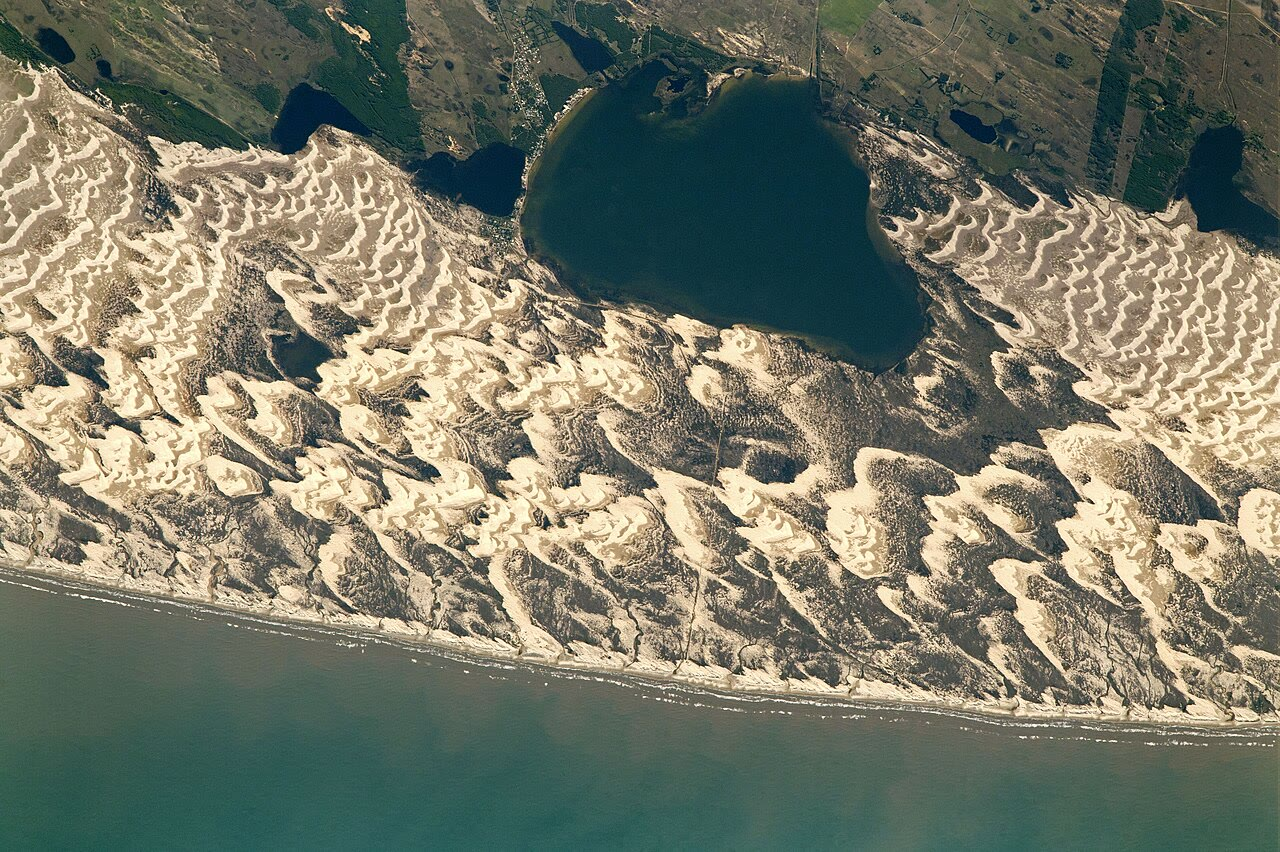
\includegraphics[width=\linewidth]{images/book1/g9-barchans.jpg}
\end{minipage}\hfill
\begin{minipage}[c]{0.46\linewidth}\raggedright
{\small दक्षिणी ब्राज़ील के अटलांटिक \omterm{def:g1:landscapes-around-us:water}{तट} पर अर्धचंद्राकार \omterm{def:g9:landforms:dune}{टिब्बे}, 2017 में अंतर्राष्ट्रीय
अंतरिक्ष स्टेशन से एक अंतरिक्ष यात्री द्वारा खींचे गए। गहरे रंग की \omterm{def:g1:landscapes-around-us:water}{झील}, लागोआ दोस बारोस,
लगभग \qty{4.5}{km} लंबी है। \omterm{def:g3:stones-pebbles-sand:sand}{रेत} फ़ोटो के निचले हिस्से में दिखते \omterm{def:g9:landforms:beach}{पुलिन} से आती है। NASA
(सार्वजनिक डोमेन,
विकिमीडिया कॉमन्स के ज़रिए)।}
\end{minipage}
% ledger: commons:iss-barchans
\label{fig:g9:landforms:barchans-photo}
\end{omfigure}

किसी \omterm{def:g1:landscapes-around-us:water}{तट} पर \omterm{def:g9:landforms:beach}{पुलिन} के पीछे \omterm{def:g9:landforms:dune}{टिब्बों} की एक पंक्ति अपने पीछे की ज़मीन को तूफ़ानी लहरों से बचाती है।
\omterm{def:g9:landforms:dune}{टिब्बों} पर उगने वाले पौधे अपनी जड़ों से \omterm{def:g3:stones-pebbles-sand:sand}{रेत} को थामे रखते हैं: जहाँ उन्हें रौंदा या हटाया जाता
है, वहाँ हवा \omterm{def:g3:stones-pebbles-sand:sand}{रेत} को फिर से ले जाती है।
% ledger: nps:aeolian

\section{समुद्र से बने स्थलरूप}

\subsection{कगारें}

\begin{definition}[कगार]\label{def:g9:landforms:cliff}
\emph{कगार}\index{कगार} \omterm{def:g3:stones-pebbles-sand:rock}{चट्टान} का एक खड़ा या ऊर्ध्वाधर फलक है। किसी \omterm{def:g1:landscapes-around-us:water}{तट} पर कगार
लहरों से कटती है, जो उसके तल पर हमला करती हैं और उसे ज़मीन की ओर पीछे
हटाती हैं।
\end{definition}

लहरें \omterm{def:g9:landforms:cliff}{कगार} के तल पर पानी, \omterm{def:g3:stones-pebbles-sand:sand}{रेत} और \omterm{def:g3:stones-pebbles-sand:pebble}{कंकड़} फेंकती हैं। धीरे-धीरे वे उसके आधार में, भाटे और ज्वार
के स्तरों के बीच, एक खोखला, एक \emph{खाँच}, काट देती हैं। ऊपर की \omterm{def:g3:stones-pebbles-sand:rock}{चट्टान} आगे लटक जाती
है; \omterm{def:g4:clouds-rain-snow:precipitation}{बारिश} और पाला उसे और कमज़ोर करते हैं। एक दिन लटका हुआ हिस्सा गिर जाता है। लहरें गिरे
हुए खंडों को तोड़कर बहा ले जाती हैं, और हमला एक नए फलक पर, ज़मीन की ओर थोड़ा और अंदर,
फिर शुरू होता है। अपने पीछे \omterm{def:g9:landforms:cliff}{कगार} \omterm{def:g3:stones-pebbles-sand:rock}{चट्टान} का एक समतल चबूतरा छोड़ जाती है, \emph{तरंग-घर्षित
चबूतरा}\index{तरंग-घर्षित चबूतरा}, जो भाटे के समय दिखाई देता
है।
% ledger: nt:birling-2014, sdnp:birling

नरम \omterm{def:g3:stones-pebbles-sand:rock}{चट्टानें} सबसे तेज़ी से पीछे हटती हैं। बर्लिंग गैप पर खड़िया की \omterm{def:g9:landforms:cliff}{कगारें} हर वर्ष लगभग एक
मीटर तक खो देती हैं; पर पीछे हटना छलाँगों में होता है, एक बार में एक गिराव, और एक तूफ़ानी
जाड़ा एक साथ कई वर्षों का पीछे हटना ले जा सकता है। 1999 में पास की \omterm{def:g9:landforms:cliff}{कगारों} के ऊपर 1832 में
बने पुराने बेल टूट प्रकाशस्तंभ को, एक ही टुकड़े में, किनारे से \qty{17}{m} पीछे खिसकाया
गया, क्योंकि \omterm{def:g9:landforms:cliff}{कगार} बहुत पास आ रही
थी।
% ledger: sdnp:birling, nt:birling-2014

\begin{omfigure}
\begin{tikzpicture}[font=\footnotesize, >={Stealth[length=2mm]}]
  % panel 1: the notch
  \begin{scope}
    \fill[omSea!45] (0,-0.1) rectangle (1.8,0.75);
    \fill[omSea!45] (1.8,0.35) -- (2.25,0.55) -- (1.8,0.95) -- cycle;
    \fill[black!8] (1.6,-0.1) -- (1.8,0.25) -- (1.8,0.35) -- (2.25,0.55) -- (1.8,0.95) -- (1.8,2.4) -- (3.6,2.4) -- (3.6,-0.6) -- (0,-0.6) -- (0,-0.1) -- cycle;
    \draw[black!70] (0,-0.1) -- (1.6,-0.1) -- (1.8,0.25) -- (1.8,0.35) -- (2.25,0.55) -- (1.8,0.95) -- (1.8,2.4) -- (3.6,2.4);
    \foreach \y in {0.8,1.3,1.8} \draw[black!25] (1.8,\y) -- (3.6,\y);
    \fill[green!35!black!50] (1.8,2.4) rectangle (3.6,2.5);
    \draw[->, omSea!80!black, thick] (0.4,0.6) -- (1.6,0.6);
    \node[anchor=south, align=center] at (0.9,0.8) {लहरें};
    \draw[black!70] (2.15,0.55) -- (2.9,1.0) node[anchor=west, fill=white, inner sep=1pt] {खाँच};
    \node[anchor=north, align=center] at (1.8,-0.7) {1. लहरें एक खाँच\\काटती हैं};
    \node[anchor=south, font=\footnotesize] at (2.7,2.5) {खड़िया};
  \end{scope}
  % panel 2: collapse
  \begin{scope}[xshift=4.6cm]
    \fill[omSea!45] (0,-0.1) rectangle (2.2,0.75);
    \fill[black!8] (2.0,-0.1) -- (2.2,0.25) -- (2.25,2.4) -- (3.6,2.4) -- (3.6,-0.6) -- (0,-0.6) -- (0,-0.1) -- cycle;
    \draw[black!70] (0,-0.1) -- (2.0,-0.1) -- (2.2,0.25) -- (2.25,2.4) -- (3.6,2.4);
    \draw[black!50, dashed] (1.8,0.95) -- (1.8,2.4) -- (2.25,2.4);
    \foreach \y in {0.8,1.3,1.8} \draw[black!25] (2.25,\y) -- (3.6,\y);
    \fill[green!35!black!50] (2.25,2.4) rectangle (3.6,2.5);
    \foreach \x/\y/\s in {1.25/0.05/0.28, 1.6/0.1/0.22, 1.95/0.3/0.3, 1.45/0.35/0.18}
      \fill[black!20, draw=black!60] (\x,\y) rectangle ++(\s,\s*0.8);
    \node[anchor=north, align=center] at (1.8,-0.7) {2. लटका हुआ हिस्सा\\गिरता है};
  \end{scope}
  % panel 3: retreat and platform
  \begin{scope}[xshift=9.2cm]
    \fill[omSea!45] (0,0.2) rectangle (2.8,0.75);
    \fill[black!8] (0,0.0) -- (2.6,0.2) -- (2.8,0.3) -- (2.85,2.4) -- (4.0,2.4) -- (4.0,-0.6) -- (0,-0.6) -- cycle;
    \draw[black!70] (0,0.0) -- (2.6,0.2) -- (2.8,0.3) -- (2.85,2.4) -- (4.0,2.4);
    \foreach \y in {0.8,1.3,1.8} \draw[black!25] (2.85,\y) -- (4.0,\y);
    \fill[green!35!black!50] (2.85,2.4) rectangle (4.0,2.5);
    \draw[black!50, dashed] (1.4,0.12) -- (1.4,2.4);
    \draw[black!50, dashed] (2.1,0.16) -- (2.1,2.4);
    \draw[<-, thick] (2.8,1.6) -- (1.5,1.6);
    \node[anchor=south, align=center] at (1.4,2.45) {पुराने कगार फलक};
    \node[anchor=north, align=center] at (2.0,-0.7) {3. एक तरंग-घर्षित चबूतरा,\\भाटे पर खुला};
  \end{scope}
\end{tikzpicture}

{\small समुद्री \omterm{def:g9:landforms:cliff}{कगार} कैसे पीछे हटती है (एक रेखाचित्र, पैमाने पर नहीं)। (1) लहरें \omterm{def:g9:landforms:cliff}{कगार} के
तल पर एक खाँच काटती हैं। (2) आगे लटकी \omterm{def:g3:stones-pebbles-sand:rock}{चट्टान} गिरती है; लहरें खंडों को तोड़कर बहा ले जाती
हैं। (3) चक्र दोहराता है: \omterm{def:g9:landforms:cliff}{कगार} ज़मीन की ओर खिसकती है और अपने सामने \omterm{def:g3:stones-pebbles-sand:rock}{चट्टान} का एक समतल
चबूतरा छोड़ जाती है।}
% ledger: nt:birling-2014, sdnp:birling
\label{fig:g9:landforms:cliff-retreat}
\end{omfigure}

\begin{safety}
\omterm{def:g9:landforms:cliff}{कगार} का किनारा किसी भी पल धँस सकता है, और \omterm{def:g3:stones-pebbles-sand:rock}{चट्टानें} बिना चेतावनी के फलक से गिरती हैं। \omterm{def:g9:landforms:cliff}{कगारों}
को सुरक्षित दूरी से देखा जाता है, ऊपर किनारे से काफ़ी पीछे और नीचे \omterm{def:g9:landforms:beach}{पुलिन} पर तल से काफ़ी दूर,
और \omterm{def:g9:landforms:cliff}{कगारों} के नीचे के \omterm{def:g9:landforms:beach}{पुलिन} को ज्वार आने से पहले छोड़ दिया
जाता है।
\end{safety}
% ledger: nt:birling-2014, sdnp:birling

\subsection{पुलिन और भू-जिह्वाएँ}

\omterm{def:g9:landforms:cliff}{कगारों} से घिसी और \omterm{def:g1:landscapes-around-us:water}{नदियों} से नीचे लाई गई \omterm{def:g3:stones-pebbles-sand:sand}{रेत} और \omterm{def:g3:stones-pebbles-sand:pebble}{कंकड़} वहीं नहीं रहते जहाँ गिरते हैं: लहरें
उन्हें छाँटती हैं और \omterm{def:g1:landscapes-around-us:water}{तट} के साथ-साथ खिसकाती हैं।

\begin{definition}[पुलिन, तटीय अपवाह और भू-जिह्वा]\label{def:g9:landforms:beach}
\emph{पुलिन}\index{पुलिन} किनारे के साथ-साथ लहरों से ढेर की गई \omterm{def:g3:stones-pebbles-sand:sand}{रेत} या \omterm{def:g3:stones-pebbles-sand:pebble}{कंकड़ों} की एक
पट्टी है। जब लहरें किनारे पर तिरछी पहुँचती हैं, तो हर लहर कणों को उसी कोण पर पुलिन पर ऊपर
धकेलती है और पानी ढाल पर सीधा नीचे लौटता है: कण \omterm{def:g1:landscapes-around-us:water}{तट} के साथ-साथ टेढ़े-मेढ़े चलते हैं। किनारे
के साथ-साथ \omterm{def:g3:stones-pebbles-sand:sand}{रेत} और \omterm{def:g3:stones-pebbles-sand:pebble}{कंकड़ों} की यह गति \emph{तटीय
अपवाह}\index{तटीय अपवाह} है। \emph{भू-जिह्वा}\index{भू-जिह्वा} तटीय अपवाह से
बनी \omterm{def:g3:stones-pebbles-sand:sand}{रेत} या \omterm{def:g3:stones-pebbles-sand:pebble}{कंकड़ों} की एक लंबी, संकरी कटक है, जो एक सिरे पर ज़मीन से जुड़ी होती है और जहाँ
\omterm{def:g1:landscapes-around-us:water}{तट} मुड़ता है वहाँ \omterm{def:g2:water-on-earth:ocean}{समुद्र} में आगे निकल जाती
है।
\end{definition}
% ledger: noaa:longshore

जहाँ \omterm{def:g1:landscapes-around-us:water}{तट} मुड़ता है, किसी खाड़ी या \omterm{def:g1:landscapes-around-us:water}{नदी} के \omterm{def:g5:water-shapes-the-land:source-mouth}{मुहाने} पर, वहाँ अपवाह उसी दिशा में चलता रहता है
और अपना भार शांत पानी में गिरा देता है: \omterm{def:g9:landforms:beach}{पुलिन} \omterm{def:g9:landforms:beach}{भू-जिह्वा} के रूप में \omterm{def:g2:water-on-earth:ocean}{समुद्र} में आगे बढ़ता है।
उसका सिरा अक्सर अंदर की ओर मुड़ जाता है, दूसरी दिशाओं से आने वाली लहरों से मुड़कर।
\omterm{def:g9:landforms:beach}{भू-जिह्वा} के पीछे, लहरों से बचा, \omterm{def:g3:stones-pebbles-sand:sand}{कीचड़} बैठता है और लवण दलदल पनपते
हैं।
% ledger: noaa:longshore

\begin{omfigure}
\begin{tikzpicture}[font=\footnotesize, >={Stealth[length=2mm]}]
  % sea
  \fill[omSea!40] (0,0) rectangle (11,2.3);
  % land with a bay
  \fill[green!25!black!20] (0,2.3) -- (6,2.3) .. controls (6.3,3.0) and (7.0,3.5) .. (8.0,3.5)
     .. controls (9.0,3.5) and (9.3,2.8) .. (9.5,2.3) -- (11,2.3) -- (11,4.6) -- (0,4.6) -- cycle;
  % calm water of the bay
  \fill[omSea!20] (6,2.3) .. controls (6.3,3.0) and (7.0,3.5) .. (8.0,3.5)
     .. controls (9.0,3.5) and (9.3,2.8) .. (9.5,2.3) -- cycle;
  % salt marsh
  \fill[green!50!black!35] (6.15,2.55) .. controls (6.6,3.1) and (7.3,3.2) .. (7.9,3.0)
     .. controls (7.6,2.7) and (7.0,2.6) .. (6.15,2.55) -- cycle;
  \node[anchor=west, font=\scriptsize] at (6.5,3.85) {लवण दलदल};
  \draw[black!60] (6.9,3.75) -- (7.0,2.95);
  % river
  \draw[omRiver, line width=1.2pt] (8.6,4.6) .. controls (8.5,4.0) and (8.3,3.7) .. (8.3,3.48);
  \node[anchor=west, font=\scriptsize] at (8.65,4.25) {नदी};
  % beach
  \fill[yellow!40!orange!35] (0,1.85) rectangle (6,2.3);
  % spit
  \fill[yellow!40!orange!35] (5.9,1.85) .. controls (7.0,1.95) and (7.8,2.0) .. (8.35,2.1)
     .. controls (8.6,2.2) and (8.6,2.5) .. (8.4,2.65) -- (8.25,2.55)
     .. controls (8.35,2.45) and (8.3,2.35) .. (8.15,2.32)
     .. controls (7.5,2.28) and (6.8,2.3) .. (6.0,2.3) -- cycle;
  \draw[black!60] (0,2.3) -- (6,2.3) .. controls (6.3,3.0) and (7.0,3.5) .. (8.0,3.5)
     .. controls (9.0,3.5) and (9.3,2.8) .. (9.5,2.3) -- (11,2.3);
  % waves arriving at an angle
  \foreach \x in {0.9,2.0,3.1,4.2} \draw[omSea!70!black, line width=0.5pt] (\x,1.15) -- ++(-35:1.1);
  \draw[->, omSea!70!black, thick] (0.6,0.3) -- ++(55:1.2) node[pos=0.15, left, black] {लहरें};
  % zigzag of a pebble
  \draw[->, black, thick] (1.0,1.9) -- (1.35,2.2) -- (1.35,1.9) -- (1.7,2.2) -- (1.7,1.9)
     -- (2.05,2.2) -- (2.05,1.9) -- (2.4,2.2) -- (2.4,1.9);
  \node[anchor=south, align=center, font=\scriptsize] at (1.7,2.45) {पुलिन पर तिरछे\\ऊपर, सीधे\\नीचे वापस};
  % drift arrow
  \draw[->, line width=1.6pt, omWarm] (3.0,1.55) -- (5.6,1.55) node[midway, below, black] {तटीय अपवाह};
  % spit label
  \draw[black!70] (7.4,2.05) -- (7.6,1.2) node[anchor=north, align=center, black] {भू-जिह्वा खाड़ी के\\पार बढ़ती है};
  \draw[->, thick, omWarm] (8.6,1.95) -- ++(0.6,0);
  % compass
  \draw[->] (10.4,0.3) -- ++(0,0.6) node[above] {उ};
\end{tikzpicture}

{\small \omterm{def:g9:landforms:beach}{तटीय अपवाह} और एक \omterm{def:g9:landforms:beach}{भू-जिह्वा}, ऊपर से देखे गए (एक रेखाचित्र)। लहरें दक्षिण-पश्चिम से
आती हैं; हर लहर \omterm{def:g3:stones-pebbles-sand:sand}{रेत} और \omterm{def:g3:stones-pebbles-sand:pebble}{कंकड़ों} को \omterm{def:g9:landforms:beach}{पुलिन} पर तिरछे ऊपर धकेलती है, और पानी सीधा नीचे लौटता
है: कण टेढ़े-मेढ़े पूर्व की ओर चलते हैं। जहाँ \omterm{def:g1:landscapes-around-us:water}{तट} एक खाड़ी में मुड़ता है, वहाँ अपवाह चलता रहता
है और एक \omterm{def:g9:landforms:beach}{भू-जिह्वा} बनाता है, जिसके पीछे एक लवण दलदल पनपता है। \omterm{def:g1:landscapes-around-us:water}{नदी} \omterm{def:g9:landforms:beach}{भू-जिह्वा} के सिरे पर एक
धारा-मार्ग खुला रखती
है।}
% ledger: noaa:longshore
\label{fig:g9:landforms:spit}
\end{omfigure}

\begin{omfigure}
\begin{minipage}[c]{0.5\linewidth}\centering
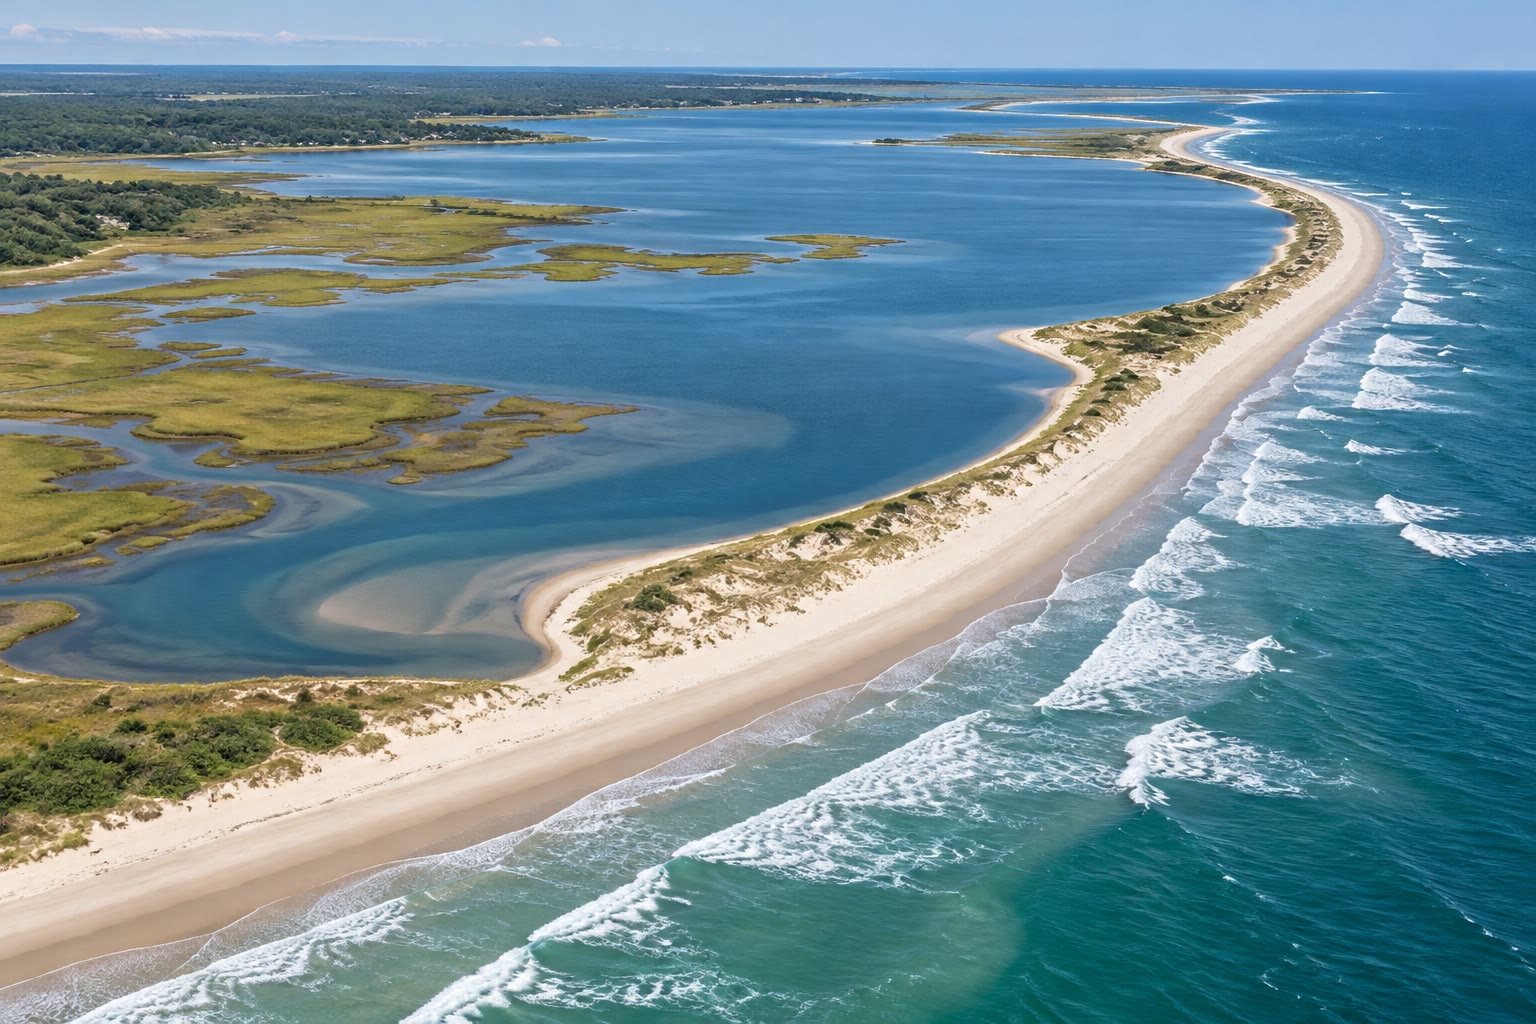
\includegraphics[width=\linewidth]{images/book1/ai/g9-spit-aerial.jpg}
\end{minipage}\hfill
\begin{minipage}[c]{0.46\linewidth}\raggedright
{\small किसी खाड़ी के \omterm{def:g5:water-shapes-the-land:source-mouth}{मुहाने} के पार एक रेतीली \omterm{def:g9:landforms:beach}{भू-जिह्वा}, एक नीचे उड़ते विमान से देखी गई
(एक चित्रण, कोई असली जगह नहीं)। लहरें उसके \omterm{def:g2:water-on-earth:ocean}{समुद्र} की ओर वाले \omterm{def:g9:landforms:beach}{पुलिन} पर टूटती हैं; उसके पीछे
शांत पानी और लवण दलदल हैं।}
\end{minipage}
\label{fig:g9:landforms:spit-ai}
\end{omfigure}

\section{घुलने से बने स्थलरूप: कार्स्ट}

\omterm{def:g4:clouds-rain-snow:precipitation}{बारिश} का पानी शुद्ध पानी नहीं है। हवा से गिरते हुए और फिर मिट्टी में रिसते हुए वह कार्बन
डाइऑक्साइड ले लेता है, जो उसे हल्का-सा अम्लीय बना देती है। यह कमज़ोर अम्ल धीरे-धीरे वह
करता है जो तनु अम्ल की बूँद चूना पत्थर के एक टुकड़े पर तेज़ी से करती है: वह \omterm{def:g3:stones-pebbles-sand:rock}{चट्टान} को घोल
देता है। चूना पत्थर दरारों से भरा है, अपनी परतों के साथ-साथ भी और उन्हें काटती हुई भी। पानी
उनमें नीचे रिसता है और उन्हें, मिलीमीटर-दर-मिलीमीटर, हज़ारों वर्षों में चौड़ा करता है।
% ledger: usgs:sinkholes, nps:karst

\begin{definition}[कार्स्ट, गुफा और घोलरंध्र]\label{def:g9:landforms:karst}
\emph{कार्स्ट}\index{कार्स्ट} एक ऐसा \omterm{def:g1:landscapes-around-us:landscape}{भूदृश्य} है जिसे किसी घुलनशील \omterm{def:g3:stones-pebbles-sand:rock}{चट्टान}, ज़्यादातर चूना
पत्थर, को घोलते पानी ने आकार दिया है। वहाँ \omterm{def:g1:landscapes-around-us:water}{नदियाँ} ज़मीन के नीचे ग़ायब हो जाती हैं और \omterm{def:g6:water-underground:spring}{सोतों} के
रूप में बाहर लौट आती हैं। \emph{गुफा}\index{गुफा} ज़मीन के नीचे की एक प्राकृतिक जगह है
जो इतनी बड़ी हो कि उसमें कोई व्यक्ति घुस सके, जो \omterm{def:g3:stones-pebbles-sand:rock}{चट्टान} की दरारों के साथ-साथ घुलकर बनी है।
\emph{घोलरंध्र}\index{घोलरंध्र} ज़मीन की सतह में एक गड्ढा या छेद है, जो वहाँ बनता है जहाँ
नीचे की \omterm{def:g3:stones-pebbles-sand:rock}{चट्टान} घुलकर निकल जाती है या जहाँ किसी गुफा की छत धँस जाती
है।
\end{definition}
% ledger: nps:karst, usgs:sinkholes

\begin{omfigure}
\begin{tikzpicture}[x=0.9cm, y=0.9cm, font=\footnotesize, >={Stealth[length=2mm]}]
  \pic (B) at (0,0) {blockdiagram={10}{4}{4}};
  % top face: grassland
  \fill[green!25!black!18] (B-ftl) -- (B-ftr) -- (B-btr) -- (B-btl) -- cycle;
  % right face
  \fill[omLithLime!70] (B-fbr) -- (B-bbr) -- (B-btr) -- (B-ftr) -- cycle;
  % front face: limestone layers
  \fill[omLithLime] (B-fbl) rectangle (B-ftr);
  \foreach \y in {0.8,1.6,2.4,3.2} \draw[black!35] (0,\y) -- (10,\y);
  \foreach \x/\y in {1.2/0.8, 3.1/1.6, 4.6/0, 6.8/2.4, 8.3/0.8, 2.2/2.4, 9.1/2.4, 5.6/3.2}
    \draw[black!35] (\x,\y) -- ++(0,0.8);
  % soil
  \fill[brown!45] (0,3.8) rectangle (10,4);
  % sinkhole on the top face and in the front face
  \fill[green!25!black!35] (3.0,4.45) ellipse (0.7 and 0.22);
  \fill[white] (2.3,4) -- (3.7,4) -- (3.25,3.45) -- (2.75,3.45) -- cycle;
  \fill[green!25!black!30] (2.3,4) -- (3.7,4) -- (3.25,3.45) -- (2.75,3.45) -- cycle;
  \draw[black!60] (2.3,4) -- (2.75,3.45) -- (3.25,3.45) -- (3.7,4);
  % shaft from sinkhole to cave
  \fill[white] (2.85,3.45) -- (3.15,3.45) -- (3.35,2.0) -- (3.05,2.0) -- cycle;
  \draw[black!60] (2.85,3.45) -- (3.05,2.0) (3.15,3.45) -- (3.35,2.0);
  % cave
  \fill[white] (2.6,2.1) .. controls (3.5,2.35) and (5.5,2.3) .. (6.6,1.9)
     .. controls (7.4,1.6) and (7.6,1.2) .. (7.2,1.0)
     .. controls (6.0,0.85) and (4.0,1.0) .. (3.0,1.2)
     .. controls (2.3,1.35) and (2.1,1.9) .. (2.6,2.1) -- cycle;
  \draw[black!70] (2.6,2.1) .. controls (3.5,2.35) and (5.5,2.3) .. (6.6,1.9)
     .. controls (7.4,1.6) and (7.6,1.2) .. (7.2,1.0)
     .. controls (6.0,0.85) and (4.0,1.0) .. (3.0,1.2)
     .. controls (2.3,1.35) and (2.1,1.9) .. (2.6,2.1);
  % underground stream at the cave floor
  \fill[omRiver!60] (3.0,1.2) .. controls (4.0,1.0) and (6.0,0.85) .. (7.2,1.0) -- (7.1,1.12)
     .. controls (6.0,1.0) and (4.0,1.12) .. (3.1,1.3) -- cycle;
  % stalactites and stalagmites
  \foreach \x/\l in {4.2/0.35, 4.5/0.22, 4.9/0.4, 5.3/0.25, 5.8/0.3}
    \fill[black!45] (\x-0.07,2.22) -- (\x+0.06,2.22) -- (\x,2.22-\l) -- cycle;
  \foreach \x/\l in {4.9/0.3, 5.8/0.25}
    \fill[black!45] (\x-0.12,0.95) -- (\x+0.12,0.95) -- (\x,0.95+\l) -- cycle;
  % disappearing stream on the top face
  \draw[omRiver, line width=1.2pt] (7.4,4.85) .. controls (6.9,4.5) and (6.4,4.4) .. (6.0,4.25);
  \fill[black!70] (6.0,4.25) circle (0.07);
  \draw[omRiver, dashed, thick] (6.0,4.0) -- (6.4,2.1);
  % spring on the right face
  \draw[omRiver, line width=1.2pt, ->] (10.2,1.2) .. controls (10.8,1.1) and (11.2,0.7) .. (11.6,0.5);
  % rain with carbon dioxide
  \foreach \x in {0.6,1.2,1.8} \draw[->, omRiver] (\x,5.6) -- ++(-0.15,-0.7);
  \draw[->, omRiver, dashed] (1.0,3.9) -- (1.2,1.7);
  % outline
  \draw[black!70] (B-fbl) rectangle (B-ftr);
  \draw[black!70] (B-ftl) -- (B-btl) -- (B-btr) -- (B-ftr) (B-btr) -- (B-bbr) -- (B-fbr);
  % labels
  \node[anchor=south, align=center] at (1.2,5.6) {बारिश कार्बन डाइऑक्साइड\\लेती है: हल्की अम्लीय};
  \node[anchor=east, align=right] at (-0.1,1.6) {पानी दरारों को\\चौड़ा करता है};
  \draw[black!70] (-0.05,1.6) -- (1.1,2.0);
  \node[anchor=south] at (3.0,5.2) {घोलरंध्र};
  \draw[black!70] (3.0,5.2) -- (3.0,4.55);
  \node[anchor=south, align=center] at (7.6,5.3) {एक धारा ज़मीन के\\नीचे ग़ायब होती है};
  \draw[black!70] (7.0,5.3) -- (6.1,4.35);
  \node[anchor=north, align=center] at (5.0,-0.1) {एक गुफा: आश्चुताश्म छत से लटकते हैं,\\निश्चुताश्म फ़र्श से उठते हैं};
  \draw[black!70] (5.0,-0.1) -- (5.0,1.4);
  \node[anchor=west, align=left] at (11.6,0.6) {सोता};
  \node[anchor=west] at (11.9,3.4) {चूना पत्थर};
\end{tikzpicture}

{\small एक \omterm{def:g9:landforms:karst}{कार्स्ट} \omterm{def:g1:landscapes-around-us:landscape}{भूदृश्य} (एक रेखाचित्र, पैमाने पर नहीं)। हल्का अम्लीय पानी चूना पत्थर की
दरारों में रिसता है और उन्हें चौड़ा करता है; ज़मीन के नीचे की धाराएँ \omterm{def:g9:landforms:karst}{गुफाएँ} खोखली करती हैं;
किसी \omterm{def:g9:landforms:karst}{गुफा} की छत धँसती है और एक \omterm{def:g9:landforms:karst}{घोलरंध्र} खोल देती है; एक धारा एक छेद में ग़ायब होती है और
नीचे एक \omterm{def:g6:water-underground:spring}{सोते} के रूप में बाहर लौट आती है।}
% ledger: nps:karst, usgs:sinkholes, nps:speleothems
\label{fig:g9:landforms:karst}
\end{omfigure}

\omterm{def:g9:landforms:karst}{गुफा} में घुलना उलटा भी चल सकता है। छत से रिसती पानी की एक बूँद घुला हुआ चूना पत्थर ले
जाती है। जब वह \omterm{def:g9:landforms:karst}{गुफा} की हवा से मिलती है, तो अपनी कुछ कार्बन डाइऑक्साइड छोड़ देती है, और बूँद
के चारों ओर पानी से कैल्साइट की एक पतली परत बाहर आ जाती है। बूँद-दर-बूँद, छत से एक खोखली
नली बढ़ती है, फिर मोटी होकर \emph{आश्चुताश्म}\index{आश्चुताश्म} बन जाती है, जो बर्फ़ की
लटकती छड़ की तरह लटकता है। जहाँ बूँदें गिरती हैं, वहाँ बाक़ी कैल्साइट फ़र्श से ऊपर
\emph{निश्चुताश्म}\index{निश्चुताश्म} बनाता है। जब दोनों मिलते हैं, तो एक स्तंभ बनाते
हैं।
% ledger: nps:speleothems

\begin{omfigure}
\begin{minipage}[c]{0.5\linewidth}\centering
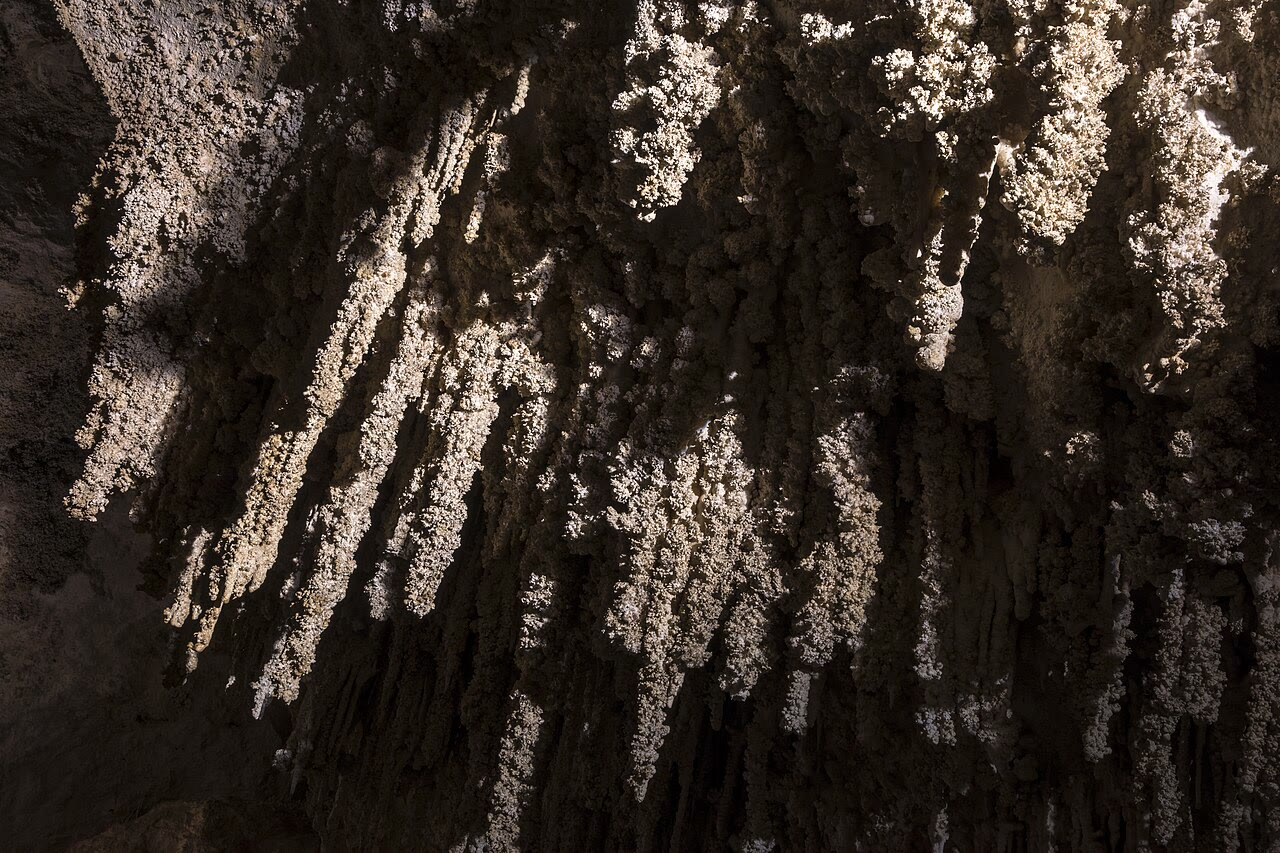
\includegraphics[width=\linewidth]{images/book1/g9-stalactites.jpg}
\end{minipage}\hfill
\begin{minipage}[c]{0.46\linewidth}\raggedright
{\small न्यू मेक्सिको की कार्ल्सबाड \omterm{def:g9:landforms:karst}{गुफा} में, जो चूना पत्थर में घुलकर बनी है, \omterm{def:g3:stones-pebbles-sand:rock}{चट्टान} के एक
बड़े खंड के नीचे लटकते आश्चुताश्म। हर एक ऊपर की \omterm{def:g3:stones-pebbles-sand:rock}{चट्टान} से रिसते पानी से बूँद-दर-बूँद
बढ़ा। अमेरिकी राष्ट्रीय उद्यान सेवा, 2018 (सार्वजनिक
डोमेन, विकिमीडिया कॉमन्स के ज़रिए)।}
\end{minipage}
% ledger: commons:carlsbad-stalactites, nps:speleothems
\label{fig:g9:landforms:stalactites}
\end{omfigure}

\omterm{def:g9:landforms:karst}{कार्स्ट} प्रदेश ज़मीन के नीचे बहुत पानी रखता है, पर वह खुली दरारों से तेज़ी से बहता है और
मुश्किल से छनता है: ज़मीन पर जो कुछ भी गिराया जाए वह जल्दी किसी \omterm{def:g6:water-underground:spring}{सोते} तक पहुँच सकता है। और
जहाँ नीचे की \omterm{def:g3:stones-pebbles-sand:rock}{चट्टान} घुल चुकी है, वहाँ ज़मीन धँस या ढह सकती है: जहाँ लोग रहते हैं, अचानक
खुलने वाला \omterm{def:g9:landforms:karst}{घोलरंध्र} सड़कों और घरों को निगल सकता
है।
% ledger: nps:karst, usgs:sinkholes

\section{भूदृश्य को पढ़ना}

हर \omterm{def:g1:landscapes-around-us:landform}{स्थलरूप} एक सुराग़ है। उसका आकार बताता है कि किस कारक ने उसे बनाया; कारक बताता है कि
कौन-सी प्रक्रिया काम कर रही थी, \omterm{def:g5:water-shapes-the-land:erosion}{अपरदन} या \omterm{def:g5:water-shapes-the-land:deposition}{निक्षेपण}; और प्रक्रिया अक्सर नीचे की \omterm{def:g3:stones-pebbles-sand:rock}{चट्टान} या
ढीले पदार्थ के बारे में कुछ बताती है।

\begin{method}[किसी स्थलरूप को पढ़ना]
\begin{enumerate}
  \item \textbf{आकार।} \omterm{def:g1:landscapes-around-us:landform}{स्थलरूप} का वर्णन करो: एक कटक, एक गड्ढा, एक खड़ा फलक, एक
        समतल चबूतरा; उसका आकार; वह किस ओर इशारा करता है।
  \item \textbf{कारक और प्रक्रिया।} तय करो कि किस कारक ने उसे बनाया (\omterm{def:g1:landscapes-around-us:water}{नदी},
        बर्फ़, हवा, \omterm{def:g2:water-on-earth:ocean}{समुद्र}, घोलता पानी) और क्या वह तराशा गया (\omterm{def:g5:water-shapes-the-land:erosion}{अपरदन}) या बनाया गया
        (\omterm{def:g5:water-shapes-the-land:deposition}{निक्षेपण})।
  \item \textbf{पदार्थ।} बताओ कि वह किससे बना है, या नीचे की \omterm{def:g3:stones-pebbles-sand:rock}{चट्टान} क्या होने की
        संभावना है: ढीली \omterm{def:g3:stones-pebbles-sand:sand}{रेत}, \omterm{def:g3:stones-pebbles-sand:pebble}{कंकड़}, चूना पत्थर, कठोर या नरम \omterm{def:g3:stones-pebbles-sand:rock}{चट्टान}।
\end{enumerate}
\end{method}

\begin{center}
{\small
\begin{tabular}{|>{\raggedright\arraybackslash}p{4.6cm}|>{\raggedright\arraybackslash}p{2.6cm}|>{\raggedright\arraybackslash}p{2.2cm}|>{\raggedright\arraybackslash}p{2.6cm}|}
\hline
आकार & कारक & प्रक्रिया & पदार्थ \\
\hline
\omterm{def:g3:stones-pebbles-sand:sand}{रेत} की अर्धचंद्राकार \omterm{def:g1:landscapes-around-us:landform}{पहाड़ियाँ} & हवा & \omterm{def:g5:water-shapes-the-land:deposition}{निक्षेपण} & ढीली \omterm{def:g3:stones-pebbles-sand:sand}{रेत} \\
समतल चट्टानी चबूतरे के ऊपर एक ऊर्ध्वाधर चट्टानी फलक & \omterm{def:g2:water-on-earth:ocean}{समुद्र} & \omterm{def:g5:water-shapes-the-land:erosion}{अपरदन} & \omterm{def:g3:stones-pebbles-sand:rock}{चट्टान} (नरम \omterm{def:g3:stones-pebbles-sand:rock}{चट्टान} तेज़ी से पीछे हटती है) \\
खाड़ी के पार \omterm{def:g3:stones-pebbles-sand:sand}{रेत} की एक संकरी कटक & \omterm{def:g2:water-on-earth:ocean}{समुद्र} (\omterm{def:g9:landforms:beach}{तटीय अपवाह}) & \omterm{def:g5:water-shapes-the-land:deposition}{निक्षेपण} & \omterm{def:g3:stones-pebbles-sand:sand}{रेत} या \omterm{def:g3:stones-pebbles-sand:pebble}{कंकड़} \\
खेतों में गड्ढे, ग़ायब होती धाराएँ & घोलता पानी & घुलना & चूना पत्थर \\
एक \omterm{def:g8:ice-on-earth:glacial-landforms}{U-आकार की घाटी} & बर्फ़ & \omterm{def:g5:water-shapes-the-land:erosion}{अपरदन} & कोई भी \omterm{def:g3:stones-pebbles-sand:rock}{चट्टान} \\
\omterm{def:g1:landscapes-around-us:water}{नदी} के \omterm{def:g5:water-shapes-the-land:source-mouth}{मुहाने} पर \omterm{def:g3:stones-pebbles-sand:sand}{कीचड़} का एक पंखा & \omterm{def:g1:landscapes-around-us:water}{नदी} & \omterm{def:g5:water-shapes-the-land:deposition}{निक्षेपण} & \omterm{def:g3:stones-pebbles-sand:sand}{कीचड़} और \omterm{def:g3:stones-pebbles-sand:sand}{रेत} \\
\hline
\end{tabular}}
\end{center}

\begin{example}[एक पठार पर सैर]
घास से ढके एक ऊँचे पठार पर कोई धारा है ही नहीं, हालाँकि वहाँ अक्सर \omterm{def:g4:clouds-rain-snow:precipitation}{बारिश} होती है। खेतों में
कुछ मीटर चौड़े गोल गड्ढे बिखरे हैं, और नीचे की \omterm{def:g1:landscapes-around-us:landform}{घाटी} में एक चट्टानी फलक के तल से एक प्रबल
\omterm{def:g6:water-underground:spring}{सोता} फूट पड़ता है। \emph{आकार}: गड्ढे, सतह पर कोई धारा नहीं, नीचे एक \omterm{def:g6:water-underground:spring}{सोता}।
\emph{कारक और प्रक्रिया}: \omterm{def:g3:stones-pebbles-sand:rock}{चट्टान} को घोलता और ज़मीन के नीचे बहता पानी। \emph{पदार्थ}:
पठार सबसे अधिक संभावना से चूना पत्थर है, और गड्ढे \omterm{def:g9:landforms:karst}{घोलरंध्र} हैं। शिक्षक द्वारा \omterm{def:g3:stones-pebbles-sand:rock}{चट्टान} के किसी
ढीले टुकड़े पर डाली गई तनु अम्ल की एक बूँद में बुलबुले
उठेंगे।
\end{example}
% ledger: nps:karst, usgs:sinkholes

\section{अभ्यास}

\begin{exercise}[$\star$]\label{exo:g9:landforms:1}
हर \omterm{def:g1:landscapes-around-us:landform}{स्थलरूप} किस कारक ने बनाया: हवा, \omterm{def:g2:water-on-earth:ocean}{समुद्र}, \omterm{def:g1:landscapes-around-us:water}{नदी}, बर्फ़, या \omterm{def:g3:stones-pebbles-sand:rock}{चट्टान} को घोलता पानी?
(क) किसी \omterm{def:g5:weather-and-climate:desert}{मरुस्थल} में \omterm{def:g3:stones-pebbles-sand:sand}{रेत} की एक अर्धचंद्राकार \omterm{def:g1:landscapes-around-us:landform}{पहाड़ी}। (ख) आश्चुताश्मों से भरी एक \omterm{def:g9:landforms:karst}{गुफा}।
(ग) किसी खाड़ी के \omterm{def:g5:water-shapes-the-land:source-mouth}{मुहाने} के पार \omterm{def:g3:stones-pebbles-sand:pebble}{कंकड़ों} की एक लंबी कटक। (घ) एक \omterm{def:g8:ice-on-earth:glacial-landforms}{U-आकार की घाटी} जिसके
सिरे पर एक \omterm{def:g8:ice-on-earth:glacial-landforms}{हिमोढ़} है। (ङ) खड़िया का एक ऊर्ध्वाधर फलक जिसके तल पर \omterm{def:g3:stones-pebbles-sand:rock}{चट्टान} का एक समतल चबूतरा
है। (च) एक \omterm{def:g5:water-shapes-the-land:delta}{डेल्टा}।
\end{exercise}

\begin{exercise}[$\star$]\label{exo:g9:landforms:2}
हर वर्णन के लिए शब्द बताओ। (क) किसी क्षेत्र की \omterm{def:g3:stones-pebbles-sand:rock}{चट्टानों} और ज़मीन का धीमा ऊपर उठना।
(ख) किसी \omterm{def:g9:landforms:dune}{टिब्बे} की खड़ी तरफ़, हवा से दूर वाली। (ग) ज़मीन में एक छेद, जो वहाँ बना जहाँ नीचे की
\omterm{def:g3:stones-pebbles-sand:rock}{चट्टान} घुल गई है या किसी \omterm{def:g9:landforms:karst}{गुफा} की छत धँस गई है। (घ) किनारे के साथ-साथ \omterm{def:g3:stones-pebbles-sand:sand}{रेत} और \omterm{def:g3:stones-pebbles-sand:pebble}{कंकड़ों} की गति।
(ङ) चूना पत्थर को घोलते पानी से आकार पाया एक \omterm{def:g1:landscapes-around-us:landscape}{भूदृश्य}।
\end{exercise}

\begin{exercise}[$\star$]\label{exo:g9:landforms:3}
सही या ग़लत? ग़लत वाक्यों को सुधारो। (क) अर्धचंद्राकार \omterm{def:g9:landforms:dune}{टिब्बे} की भुजाएँ हवा की ओर इशारा करती
हैं। (ख) \omterm{def:g9:landforms:dune}{टिब्बे} की हवा की ओर वाली ढाल हल्की होती है। (ग) \omterm{def:g9:landforms:dune}{टिब्बा} इसलिए चलता है क्योंकि हवा
उसे एक साथ पूरा उठा लेती है। (घ) \omterm{def:g9:landforms:dune}{टिब्बे} वहाँ ज़्यादा आसानी से बनते हैं जहाँ कम पौधे
उगते हैं।
\end{exercise}

\begin{exercise}[$\star$]\label{exo:g9:landforms:4}
समुद्री \omterm{def:g9:landforms:cliff}{कगार} के पीछे हटने के इन चरणों को क्रम में रखो। (क) लहरें गिरे हुए खंडों को तोड़कर
बहा ले जाती हैं। (ख) लहरें \omterm{def:g9:landforms:cliff}{कगार} के तल पर एक खाँच काटती हैं। (ग) \omterm{def:g9:landforms:cliff}{कगार} का फलक अब ज़मीन की
ओर और अंदर खड़ा है, और उसके सामने का समतल चबूतरा थोड़ा और चौड़ा है। (घ) खाँच के ऊपर की
\omterm{def:g3:stones-pebbles-sand:rock}{चट्टान} आगे लटकती है। (ङ) लटका हुआ हिस्सा गिरता
है।
\end{exercise}

\begin{exercise}[$\star\star$]\label{exo:g9:landforms:5}
% ledger: nps:whsa-migration (6 and 3 m a year)
एक विमान से देखने पर किसी \omterm{def:g5:weather-and-climate:desert}{मरुस्थल} के सभी अर्धचंद्राकार \omterm{def:g9:landforms:dune}{टिब्बों} की भुजाएँ पूर्व की ओर इशारा
करती हैं। (क) हवा किस दिशा से चलती है? (ख) हर \omterm{def:g9:landforms:dune}{टिब्बे} के किस ओर \omterm{def:g9:landforms:dune}{फिसलन फलक} है? (ग) एक
सड़क एक \omterm{def:g9:landforms:dune}{टिब्बे} से \qty{60}{m} पूर्व में चलती है। \omterm{def:g9:landforms:dune}{टिब्बा} \qty{6}{m} प्रति वर्ष चलता है।
कितने वर्षों में उसका तल सड़क तक पहुँचेगा? (घ) एक बड़ा \omterm{def:g9:landforms:dune}{टिब्बा} केवल \qty{3}{m} प्रति
वर्ष चलता है। बड़े \omterm{def:g9:landforms:dune}{टिब्बे} ज़्यादा धीरे क्यों चलते
हैं?
\end{exercise}

\begin{exercise}[$\star\star$]\label{exo:g9:landforms:6}
% ledger: sdnp:birling, nt:birling-2014
किसी \omterm{def:g1:landscapes-around-us:water}{तट} की खड़िया की \omterm{def:g9:landforms:cliff}{कगारें} हर वर्ष लगभग \qty{1}{m} तक पीछे हटती हैं। 2014 के जाड़े में
उन्होंने केवल दो महीनों में उतना खो दिया जितना वे आमतौर पर सात वर्षों में खोती हैं।
(क) \qty{1}{m} प्रति वर्ष पर सात वर्षों में कितना खोता है? (ख) दो महीने एक वर्ष का कितना
भाग हैं? (ग) उन दो महीनों में \omterm{def:g9:landforms:cliff}{कगारें} सामान्य से कितने गुना तेज़ी से पीछे हटीं? (घ) खाँच और
लटके हुए हिस्से का उपयोग करके समझाओ कि \omterm{def:g9:landforms:cliff}{कगार} सहज रूप से नहीं, बल्कि छलाँगों में पीछे क्यों
हटती
है।
\end{exercise}

\begin{exercise}[$\star\star$]\label{exo:g9:landforms:7}
एक सीधा \omterm{def:g1:landscapes-around-us:water}{तट} पश्चिम--पूर्व चलता है, \omterm{def:g2:water-on-earth:ocean}{समुद्र} दक्षिण में है। लहरें दक्षिण-पश्चिम से आती हैं।
(क) \omterm{def:g9:landforms:beach}{तटीय अपवाह} \omterm{def:g3:stones-pebbles-sand:sand}{रेत} को किस दिशा में ले जाता है? (ख) तीन लहरों में एक \omterm{def:g3:stones-pebbles-sand:pebble}{कंकड़} का टेढ़ा-मेढ़ा
रास्ता बनाओ, \omterm{def:g9:landforms:beach}{पुलिन} पर ऊपर की चाल और नीचे वापसी की चाल पर नाम लिखकर। (ग) अपने पूर्वी
सिरे पर \omterm{def:g1:landscapes-around-us:water}{तट} उत्तर की ओर एक खाड़ी में मुड़ता है। वहाँ कौन-सा \omterm{def:g1:landscapes-around-us:landform}{स्थलरूप} बढ़ने की संभावना है?
(घ) उसके पीछे \omterm{def:g3:stones-pebbles-sand:sand}{कीचड़} क्यों बैठता
है?
\end{exercise}

\begin{exercise}[$\star\star$]\label{exo:g9:landforms:8}
(क) \omterm{def:g4:clouds-rain-snow:precipitation}{बारिश} के पानी को हल्का अम्लीय क्या बनाता है? (ख) चूना पत्थर में \omterm{def:g9:landforms:karst}{गुफाएँ} क्यों होती हैं पर
ग्रेनाइट में लगभग नहीं? (ग) \omterm{def:g9:landforms:karst}{गुफाएँ} \omterm{def:g3:stones-pebbles-sand:rock}{चट्टान} की दरारों और परतों के साथ-साथ क्यों चलती हैं?
(घ) \omterm{def:g9:landforms:karst}{घोलरंध्र} बनने के दो तरीक़े बताओ।
\end{exercise}

\begin{exercise}[$\star\star$]\label{exo:g9:landforms:9}
(क) समझाओ कि \omterm{def:g9:landforms:karst}{गुफा} की छत से लटकी पानी की बूँद से कैल्साइट क्यों बाहर आता है। (ख) युवा
आश्चुताश्मों के विपरीत, निश्चुताश्मों के अंदर कोई खोखली नली क्यों नहीं होती? (ग) मान लो कि
एक आश्चुताश्म \qty{0.1}{mm} प्रति वर्ष बढ़ा है (एक काल्पनिक दर: असली दरें बहुत बदलती
हैं)। \qty{30}{cm} बढ़ने में उसे कितने वर्ष लगे हैं? जवाब वैज्ञानिक संकेतन में
लिखो।
\end{exercise}

\begin{exercise}[$\star\star$]\label{exo:g9:landforms:10}
% ledger: usgs:himalaya, sdnp:birling
तिब्बत का पठार लगभग 10~मिलियन वर्षों में लगभग \qty{4600}{m} ऊपर उठा।
(क) औसत \omterm{def:g9:landforms:uplift}{उत्थान} मीटर प्रति वर्ष में, वैज्ञानिक संकेतन में, निकालो, फिर मिलीमीटर प्रति वर्ष
में। (ख) मान लो कि \omterm{def:g5:water-shapes-the-land:erosion}{अपरदन} पठार से हर वर्ष \qty{0.2}{mm} हटाता है (एक काल्पनिक संख्या)।
पठार हर वर्ष कितना ऊपर उठता है? (ग) खड़िया की एक \omterm{def:g9:landforms:cliff}{कगार} लगभग \qty{1}{m} प्रति वर्ष पीछे
हटती है। यह (क) के \omterm{def:g9:landforms:uplift}{उत्थान} से कितने गुना तेज़ है? (घ) एक धीमा \omterm{def:g9:landforms:uplift}{उत्थान} फिर भी एक ऊँचा पठार
क्यों बना सकता
है?
\end{exercise}

\begin{exercise}[$\star\star\star$]\label{exo:g9:landforms:11}
अध्याय की विधि (आकार, कारक और प्रक्रिया, पदार्थ) से हर \omterm{def:g1:landscapes-around-us:landscape}{भूदृश्य} को पढ़ो। (क) एक सूखे देश
में \omterm{def:g3:stones-pebbles-sand:sand}{रेत} की \omterm{def:g1:landscapes-around-us:landform}{पहाड़ियों} की लंबी पंक्तियाँ, हर एक अर्धचंद्र के आकार की, जिसकी खड़ी तरफ़
दक्षिण-पूर्व की ओर है। (ख) एक सफ़ेद \omterm{def:g9:landforms:cliff}{कगार} के तल पर, समुद्री शैवाल से ढका \omterm{def:g3:stones-pebbles-sand:rock}{चट्टान} का एक समतल
चबूतरा भाटे के समय दिखाई देता है। (ग) हल्के रंग की \omterm{def:g3:stones-pebbles-sand:rock}{चट्टान} के एक चौड़े पठार पर एक धारा
एक खेत के पार बहती है और एक छेद में ग़ायब हो जाती है; \qty{2}{km} दूर एक \omterm{def:g1:landscapes-around-us:landform}{घाटी} की
ढाल से एक \omterm{def:g6:water-underground:spring}{सोता} फूट पड़ता है।
\end{exercise}

\begin{exercise}[$\star\star\star$]\label{exo:g9:landforms:12}
% ledger: nps:whsa-migration, nmt:barchan, nps:aeolian
एक \omterm{def:g9:landforms:dune}{टिब्बा} क्षेत्र में, हवा की ओर के किनारे पर छोटे \omterm{def:g9:landforms:dune}{टिब्बे} \qty{6}{m} प्रति वर्ष तक चलते हैं;
थोड़ा आगे, 6 से \qty{10}{m} ऊँचे \omterm{def:g9:landforms:dune}{टिब्बे} लगभग \qty{3}{m} प्रति वर्ष चलते हैं। एक
पगडंडी हर तरह के एक \omterm{def:g9:landforms:dune}{टिब्बे} से हवा की दिशा में \qty{45}{m} आगे क्षेत्र को पार करती है।
(क) हर \omterm{def:g9:landforms:dune}{टिब्बा} कितने वर्षों बाद पगडंडी तक पहुँचता है? (ख) तेज़ हवाओं से धकेले गए \omterm{def:g9:landforms:dune}{टिब्बे} एक
वर्ष में \qty{100}{m} से ज़्यादा चल सकते हैं। ऐसे \omterm{def:g9:landforms:dune}{टिब्बे} को वही दूरी तय करने में कितना
समय लगेगा? (ग) \omterm{def:g9:landforms:dune}{टिब्बों} को धीमा करने का एक तरीक़ा बताओ, और समझाओ कि वह कैसे काम करता
है।
\end{exercise}

\section{समस्या: कगार और तटीय सड़क}

\begin{problem}[{सप्ताहांत समस्या --- एक तटीय सड़क पीछे हटती खड़िया की कगार के पीछे चलती
है; अंतिम उत्तर वह वर्ष है जब मापी गई दर पर कगार का किनारा सड़क तक
पहुँचेगा}]
\label{pb:g9:landforms:1}
% ledger: (invented region: exercise data, figdata/grade-9/cliff_retreat.py; the rate is kept within sdnp:birling, the storm winter recalls nt:birling-2014)
एक तटीय सड़क खड़िया की \omterm{def:g9:landforms:cliff}{कगारों} के ऊपर चलती है। हर कुछ वर्षों में एक सर्वेक्षण दल एक ही रेखा के
साथ सड़क से \omterm{def:g9:landforms:cliff}{कगार} के किनारे तक की दूरी मापता है, किनारे से काफ़ी पीछे गाड़े गए स्थिर चिह्नों
से, कभी ख़ुद किनारे पर नहीं। ये रहे उनके
माप।

\begin{center}
{\small
\begin{tabular}{|l|c|c|c|c|c|c|c|}
\hline
वर्ष & 2004 & 2008 & 2012 & 2014 & 2016 & 2020 & 2024 \\
\hline
सड़क से किनारे तक की दूरी (m) & 46.0 & 43.1 & 41.0 & 36.2 & 35.5 & 33.0 & 30.4 \\
\hline
\end{tabular}}
\end{center}

\noindent\textbf{भाग I --- माप।}\par\nopagebreak
\begin{enumerate}[beginpenalty=10000]
  \item 2004 और 2024 के बीच \omterm{def:g9:landforms:cliff}{कगार} का किनारा सड़क के कितने मीटर पास
        आया?
  \item इन 20 वर्षों में पीछे हटने की औसत दर मीटर प्रति वर्ष में
        निकालो।
  \item किन दो सर्वेक्षणों के बीच किनारा सबसे तेज़ी से पीछे हटा? उस अंतराल की दर
        निकालो।
  \item वह औसत से कितने गुना तेज़ है? सुझाव दो कि उस अंतराल में क्या
        हुआ।
\end{enumerate}

\begin{omfigure}
\begin{tikzpicture}
\begin{axis}[omrecord, width=11cm, height=4.6cm, xmin=2000, xmax=2070,
  ymin=0, ymax=50, xtick={2000,2010,...,2070}, ytick={0,10,...,50},
  x tick label style={/pgf/number format/1000 sep={}},
  xlabel={वर्ष}, ylabel={सड़क तक की दूरी (m)}]
  \addplot[omWarm, thick, mark=*, mark size=1.8pt] table[x=year, y=dist_m] {figdata/out/grade-9-cliff_retreat.dat};
\end{axis}
\end{tikzpicture}

{\small सर्वेक्षण: तटीय सड़क से \omterm{def:g9:landforms:cliff}{कगार} के किनारे तक की दूरी (अभ्यास के
आँकड़े)।}
\label{fig:g9:landforms:survey}
\end{omfigure}

\noindent\textbf{भाग II --- दर।}\par\nopagebreak
\begin{enumerate}[resume, beginpenalty=10000]
  \item औसत दर सेंटीमीटर प्रति वर्ष में लिखो, फिर मीटर प्रति
        सदी में।
  \item किसी असली खड़िया \omterm{def:g1:landscapes-around-us:water}{तट} पर \omterm{def:g9:landforms:cliff}{कगारें} हर वर्ष लगभग एक मीटर तक पीछे हटती हैं। क्या इस
        \omterm{def:g9:landforms:cliff}{कगार} का पीछे हटना उतने ही आकार का है?
  \item ऐसे ही एक \omterm{def:g1:landscapes-around-us:water}{तट} पर एक प्रकाशस्तंभ को कभी किनारे से \qty{17}{m} पीछे खिसकाया गया
        था। इस \omterm{def:g9:landforms:cliff}{कगार} की औसत दर पर \qty{17}{m} कितने वर्षों के पीछे हटने के बराबर
        है?
  \item 20 वर्षों में मापी गई दर दो वर्षों में मापी गई दर से भविष्य के लिए बेहतर मार्गदर्शक
        क्यों है?
\end{enumerate}

\noindent\textbf{भाग III --- सड़क।}\par\nopagebreak
\begin{enumerate}[resume, beginpenalty=10000]
  \item सड़क को किनारे के उससे \qty{10}{m} के भीतर आने से पहले हटाना है। औसत दर पर वह
        किस वर्ष होगा?
  \item अगर ज़्यादा तूफ़ानी जाड़े दर को दोगुना कर दें, तो किनारा किस वर्ष सड़क तक
        पहुँचेगा?
  \item सर्वेक्षण दल अपने माप किनारे से काफ़ी पीछे गाड़े गए चिह्नों से क्यों लेता है?
  \item औसत दर पर \omterm{def:g9:landforms:cliff}{कगार} का किनारा किस वर्ष सड़क तक
        पहुँचेगा?
\end{enumerate}
\end{problem}
